\section{Table of Contributions}

\begin{table}[H]
\begin{tabular}{lcccc}
\toprule
Section Name & Keiser & Krüger & Pflamminger & Wesemann  \\ 
\midrule
Introduction                                    & x & x & x & x \\
Classification in the Context of Big Data         & x & x &   &   \\
Decision Trees                                  &   & x &   &   \\
Gradient Boosting                               &   & x &   &   \\
Concepts for Data Prep...      &   &   & x &   \\
CRISP DM &   &   &   & x \\
Web APIs          &   &   & x &   \\
Basic Concepts of Music Theory                  & x &   &   &   \\
Data Collection                                 &   &   & x & x \\
Data Understanding                              &   & x &   & x \\
Data Preparation                                &   &   & x &   \\
Modeling                                        &   &   & x &   \\
Evaluation                                      & x & x &   &   \\
Conclusion                                      & x & x & x & x \\
\bottomrule
\end{tabular}
\end{table}

\newpage
\section{Data Collection Coding}
This is the complete documented code for data collection.
\label{sec:appendix_data_collection}

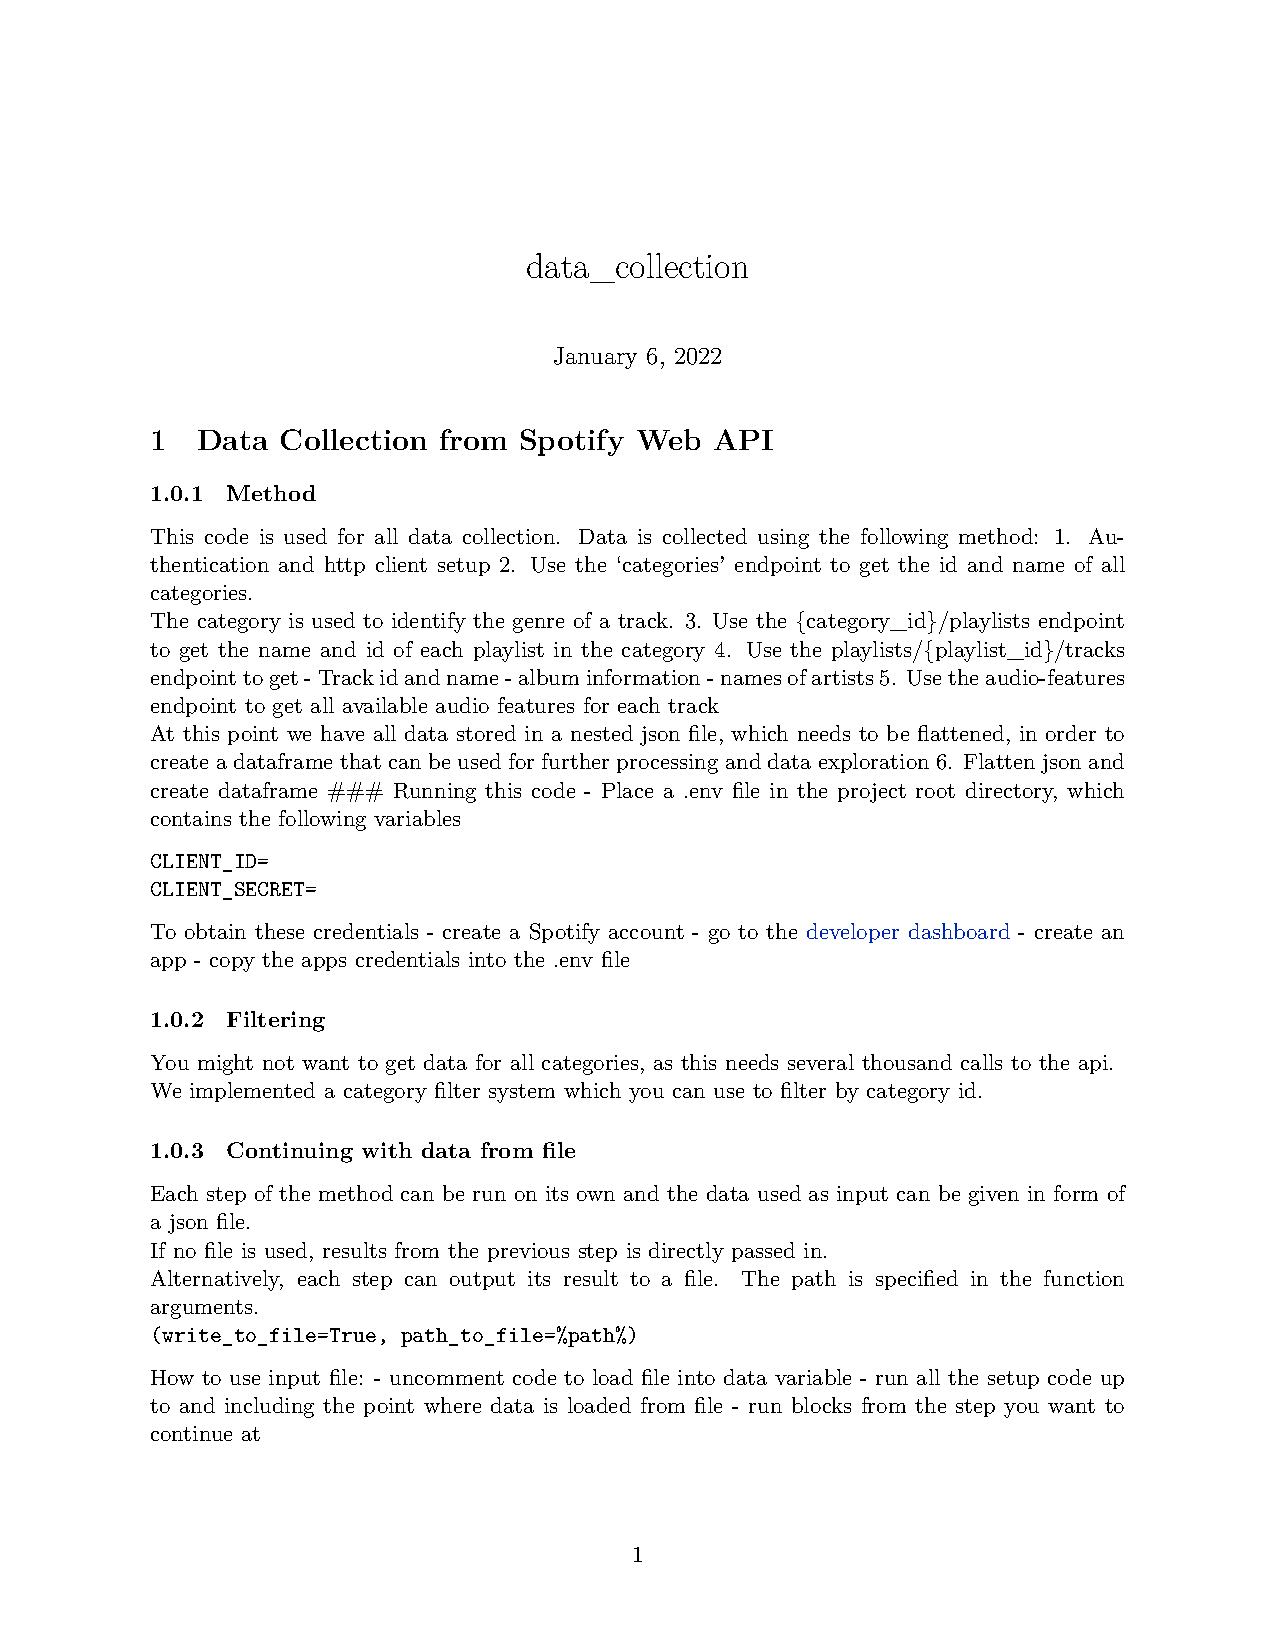
\includepdf[pages=-,frame=true,scale=0.85]{source_code/data_collection.pdf} %, offset=75 -75

\newpage
\section{Coding for CRISP DM Process}
\label{sec:appendix_crisp_dm}
This includes all code for the implementation of data understanding, preparation,
modeling and evaluation.

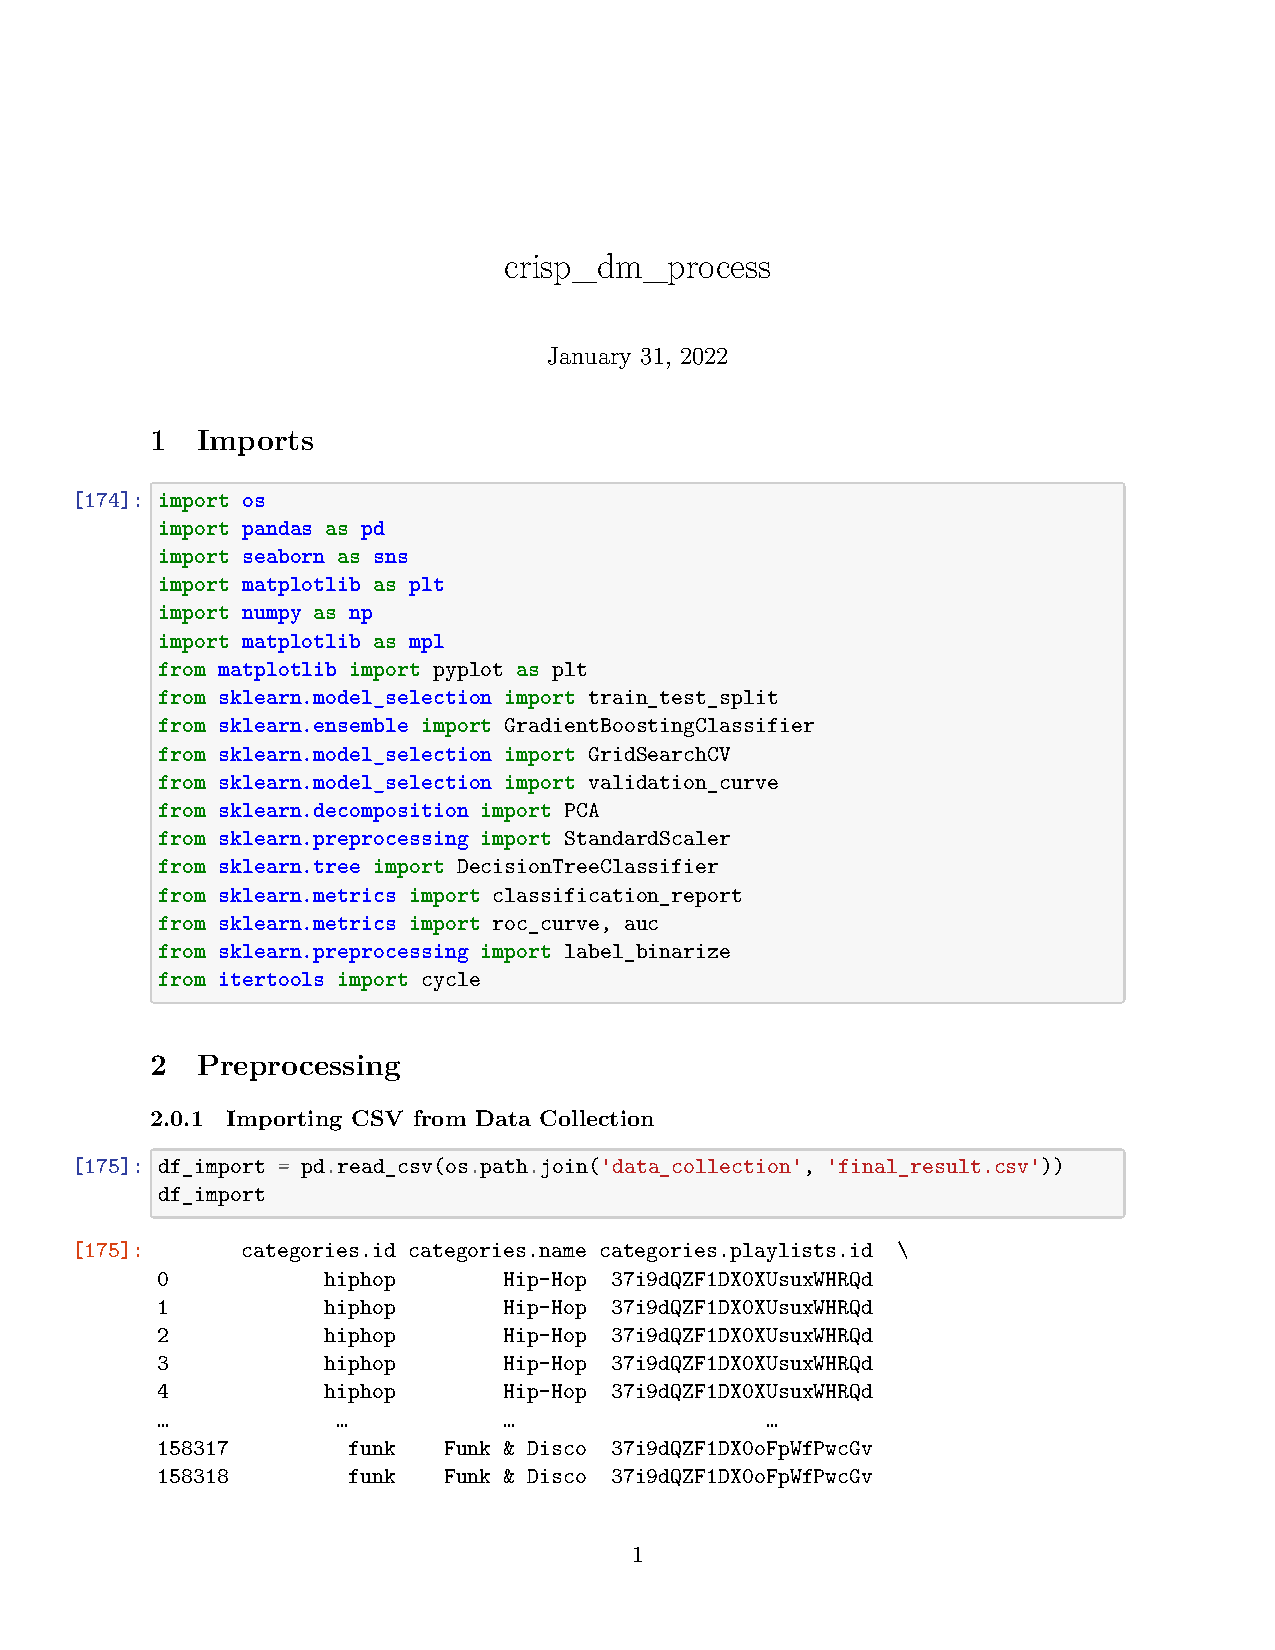
\includepdf[pages=-,frame=true,scale=0.85]{source_code/crisp_dm_process.pdf} %, offset=75 -75

\newpage
\section{Coding for Decision Tree Theory}
This is the code used to create the figures and tables for section \ref{sec:decision trees}
\label{sec:appendix_dt}

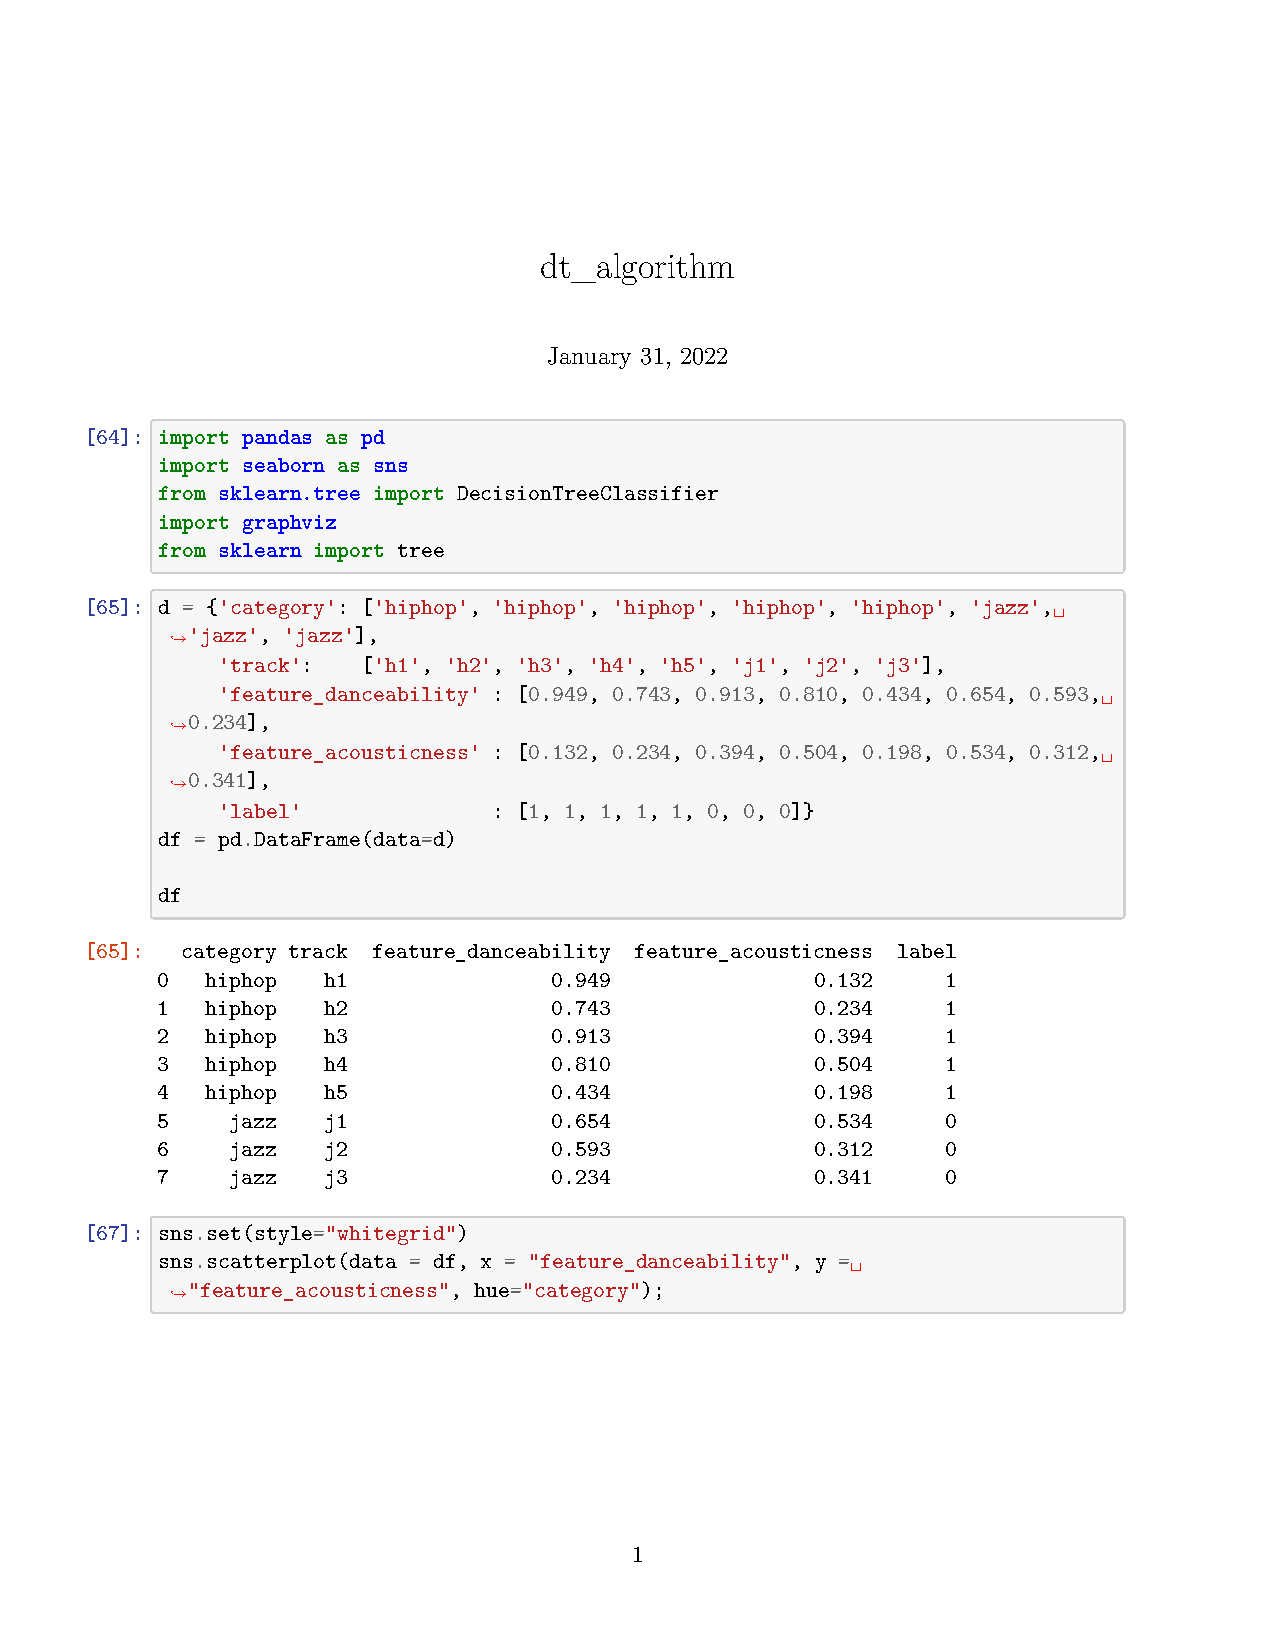
\includepdf[pages=-,frame=true,scale=0.85]{source_code/dt_algorithm.pdf} %, offset=75 -75

\newpage
\section{Coding for Gradient Boosting Theory}
This is the code used to create the figures and tables from section \ref{sec:Gradient Boosting}
\label{sec:appendix_gb}

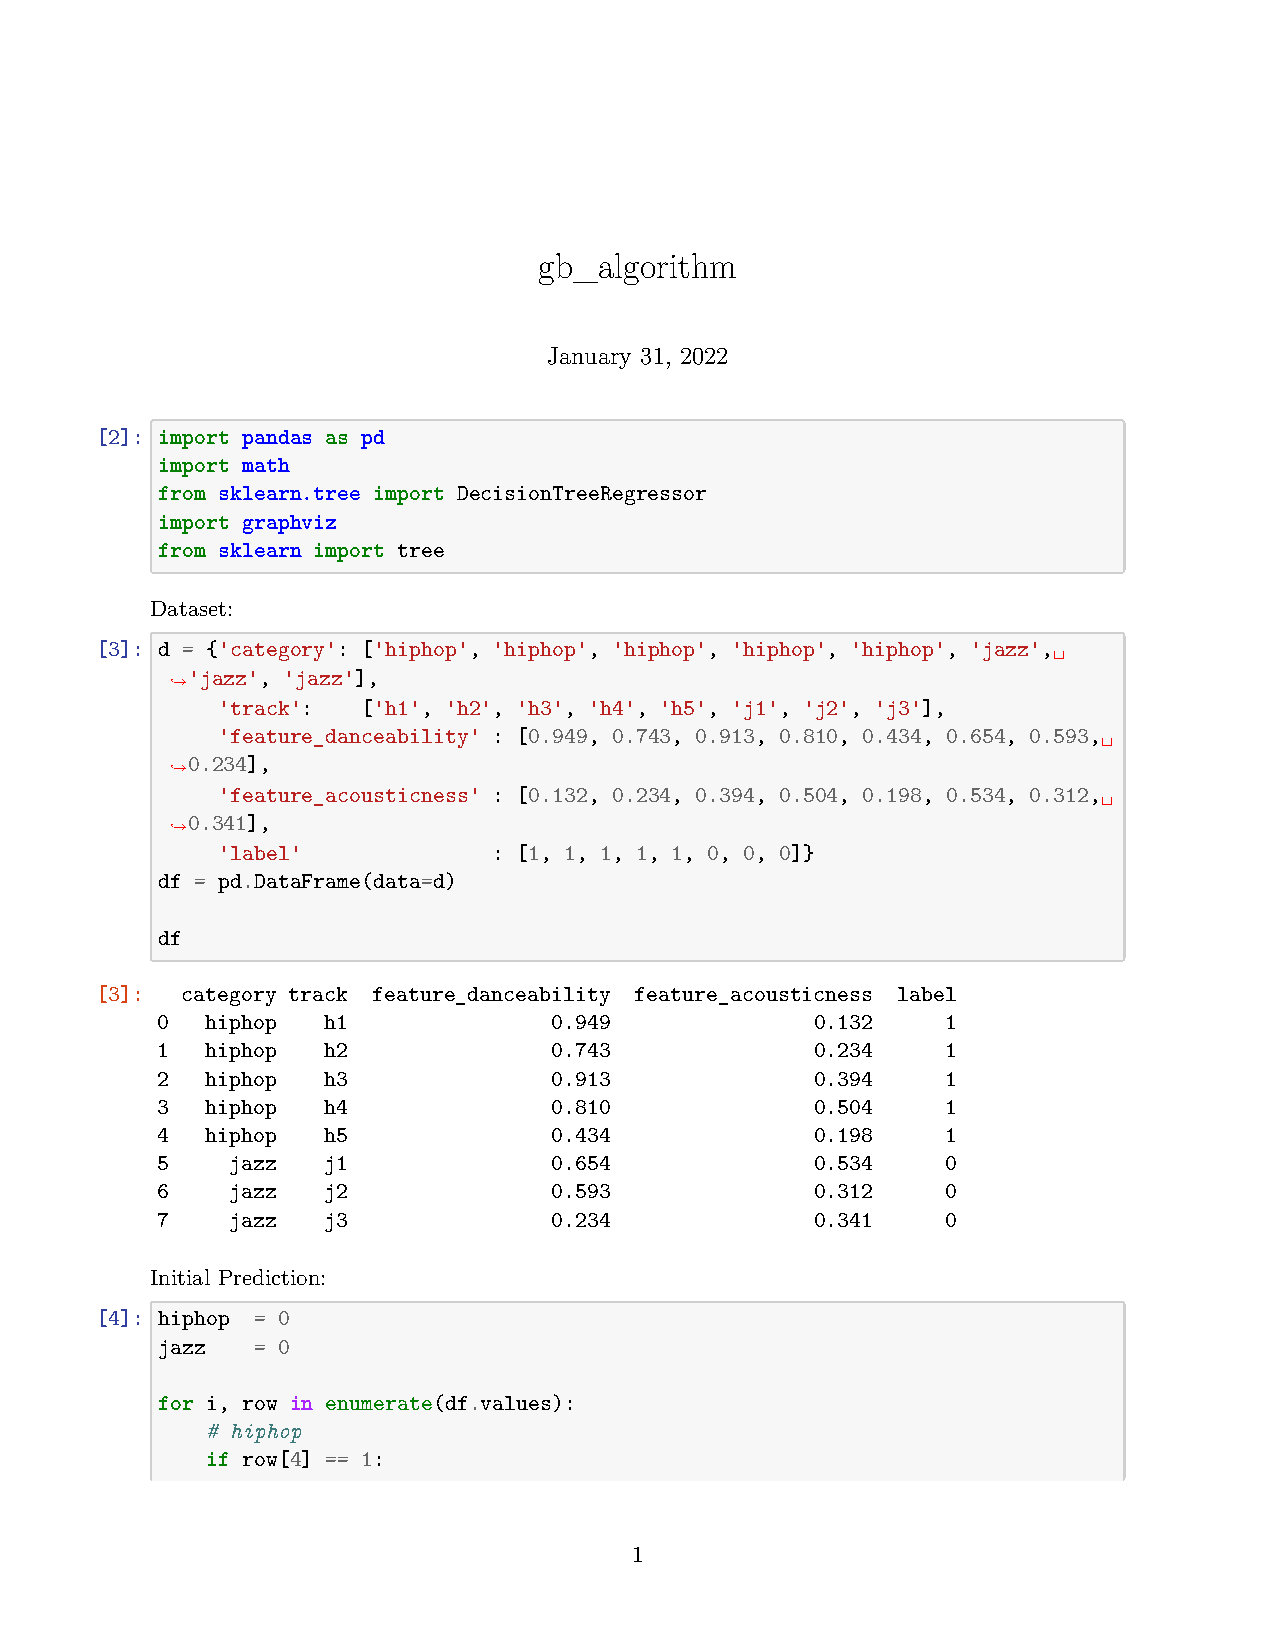
\includepdf[pages=-,frame=true,scale=0.85]{source_code/gb_algorithm.pdf} %, offset=75 -75